\chapter{Numerical Approximation of the Log-Composition}\label{ch:application_log_composition}

\begin{flushright}
	\emph{We believe that we know something about the things themselves when we speak of trees, colors, snow, and flowers; and yet we possess nothing but metaphors for things — metaphors which correspond in no way to the original entities.} \\ -Nietzsche, \emph{On Truth and Lies in extra-moral sense.}
\end{flushright}

... Group composition as a need from diffeomorphic image registration.\\
....It is of fundamental importance to have the possibility to going from an element of a group of spatial transformations  to a tangent space, in which each vector corresponds to the tangent vector field that this transformation causes on the space. It makes possible to lean on the group structure a structure of vector space, which implies the possibility to compute statistics on the group of transformation as well as compose velocity fields in the tangent space passing through the corresponding transformation (both of them are made possible thanks to the local bijection between the Lie group and the Lie algebra ). \\

% % % % % % % % % % % % % % % % % % % % % % % % % % % % % % % % % % % % % %
% % SUBSECTION
% % % % % % % % % % % % % % % % % % % % % % % % % % % % % % % % % % % % % % 
\section{Group composition at the Service of Image Registration}



% % ZZZ
We define the group composition the inner binary operation $\star$ in $\mathfrak{g}$ such that 
\begin{align*}
\star : \mathfrak{g} \times \mathfrak{g} & \longrightarrow \mathfrak{g}    \\
(\mathbf{v}_{1}, \mathbf{v}_{2}) &\longmapsto \mathbf{v}_{1}\star \mathbf{v}_{2} =  \log(\exp(\mathbf{v}_1)\circ \exp(\mathbf{v}_2))
\end{align*}
(we remember that $\circ$ is the operation of Lie group, i.e. the composition of diffeomorphism and $\exp$ and $\log$ with no subscript are the Lie exponential and Lie logarithm).\\
The \emph{offset group composition} is defined as the inner binary operation $\tilde{\star} $ over the $\mathbb{G}$ fiber bundle such that 
\begin{align*}
\tilde{\star} : T_{p_1}\mathbb{G} \times T_{p_2}\mathbb{G} & \longrightarrow T_{p_1}\mathbb{G}   
\\
(\mathbf{v}_{1}, \mathbf{v}_{2}) &\longmapsto \mathbf{v}_{1}~\tilde{\star}~ \mathbf{v}_{2}
=
\log_{p_1}(\exp_{p_2}(\mathbf{v}_{2})\circ\exp_{p_1}(\mathbf{v}_{1}))
\end{align*}
where $p_1 \in \mathbb{G}$, $p_2 = \exp_{p_1}(\mathbf{v}_{1})$ and Affine exponential and Affine logarithm are considered. Posing $p_3 = \exp_{p_2}(\mathbf{v}_{2})$ the second offset group composition is the tangent vector in $p_1$ that corresponds to the composition between $p_1$ and $p_2$, i.e. $\log_{p_1}(p_3 \circ p_2)$. \\
The BCH formula is the solution to the first kind group composition. It can be practically computed using its \emph{approximation of degree} $k$ defined as the sum of the BCH terms having no more than $k$ nested Lie bracket. For example:
\begin{align*}
BCH^{0}(\mathbf{u},\mathbf{v}) &= \mathbf{u} + \mathbf{v} \\
BCH^{1}(\mathbf{u},\mathbf{v}) &=  \mathbf{u} + \mathbf{v} + \frac{1}{2}[\mathbf{u},\mathbf{v}] \\
BCH^{2}(\mathbf{u},\mathbf{v}) &=  \mathbf{u} + \mathbf{v} + \frac{1}{2}[\mathbf{u},\mathbf{v}] + \frac{1}{12}([\mathbf{u},[\mathbf{u},\mathbf{v}]] + [\mathbf{v},[\mathbf{v},\mathbf{u}]])
\end{align*}
These numerical approximations of the group composition leave the difficulty of managing the problem of the error carried by each term. In some cases the increase of the degree of the BCH approximation do not necessarily implies a decrease in error: \\
.... Add an example in which this happens.

We present other ways to compute the Lie group composition in the following subsections.

% % % % % % % % % % % % % % % % % % % % % % % % % % % % % % % % % % % % % %
% % SUBSECTION
% % % % % % % % % % % % % % % % % % % % % % % % % % % % % % % % % % % % % % 
\section{Accelerating convergences applied to the BCH formula}

....

% % % % % % % % % % % % % % % % % % % % % % % % % % % % % % % % % % % % % %
% % SUBSECTION
% % % % % % % % % % % % % % % % % % % % % % % % % % % % % % % % % % % % % % 
\section{Taylor expansion to compute the group composition}

....


% % % % % % % % % % % % % % % % % % % % % % % % % % % % % % % % % % % % % %
% % SUBSECTION
% % % % % % % % % % % % % % % % % % % % % % % % % % % % % % % % % % % % % % 
\section{Parallel transport to compute the group composition}

....Here will be made the strong assumption according to which the parallel transport defined for the finite dimensional case, works also in the infinite dimensional case.

\begin{lemma}
	$\mathbb{G}$ Lie group, $\nabla$ connection, $a\in\mathbb{G}$, $\mathbf{u}\in T_{e}\mathbb{G}$. Let $\gamma$ be a curve defined on $\mathbb{G}$ such that $\gamma(0) = e$, $\gamma(1) = a$, $\dot{\gamma}(0) =\mathbf{u}$. Let $\beta$ be the curve over $\mathbf{G}$ defined as $\beta(t) = a\circ \gamma(t)$, then the two following conditions hold:
	\begin{enumerate}
		\item If $\nabla$ is a Cartan connection then $\beta$ is a geodesic.
		\item For $\mathbf{u}_{a} := D(L_{a})_{e}(\mathbf{u}) \in T_{a}\mathbb{G}$:
		\begin{align}
		\exp_{a}(t\mathbf{u}_{b}) = b\circ \exp_{e}( t D(L_{a^{-1}})_{a}(\mathbf{u}_{a}) ) = b\circ \exp_{e}(t\mathbf{u})
		\end{align}
	\end{enumerate}
\end{lemma}

\begin{figure}[htbp]
	\centering
	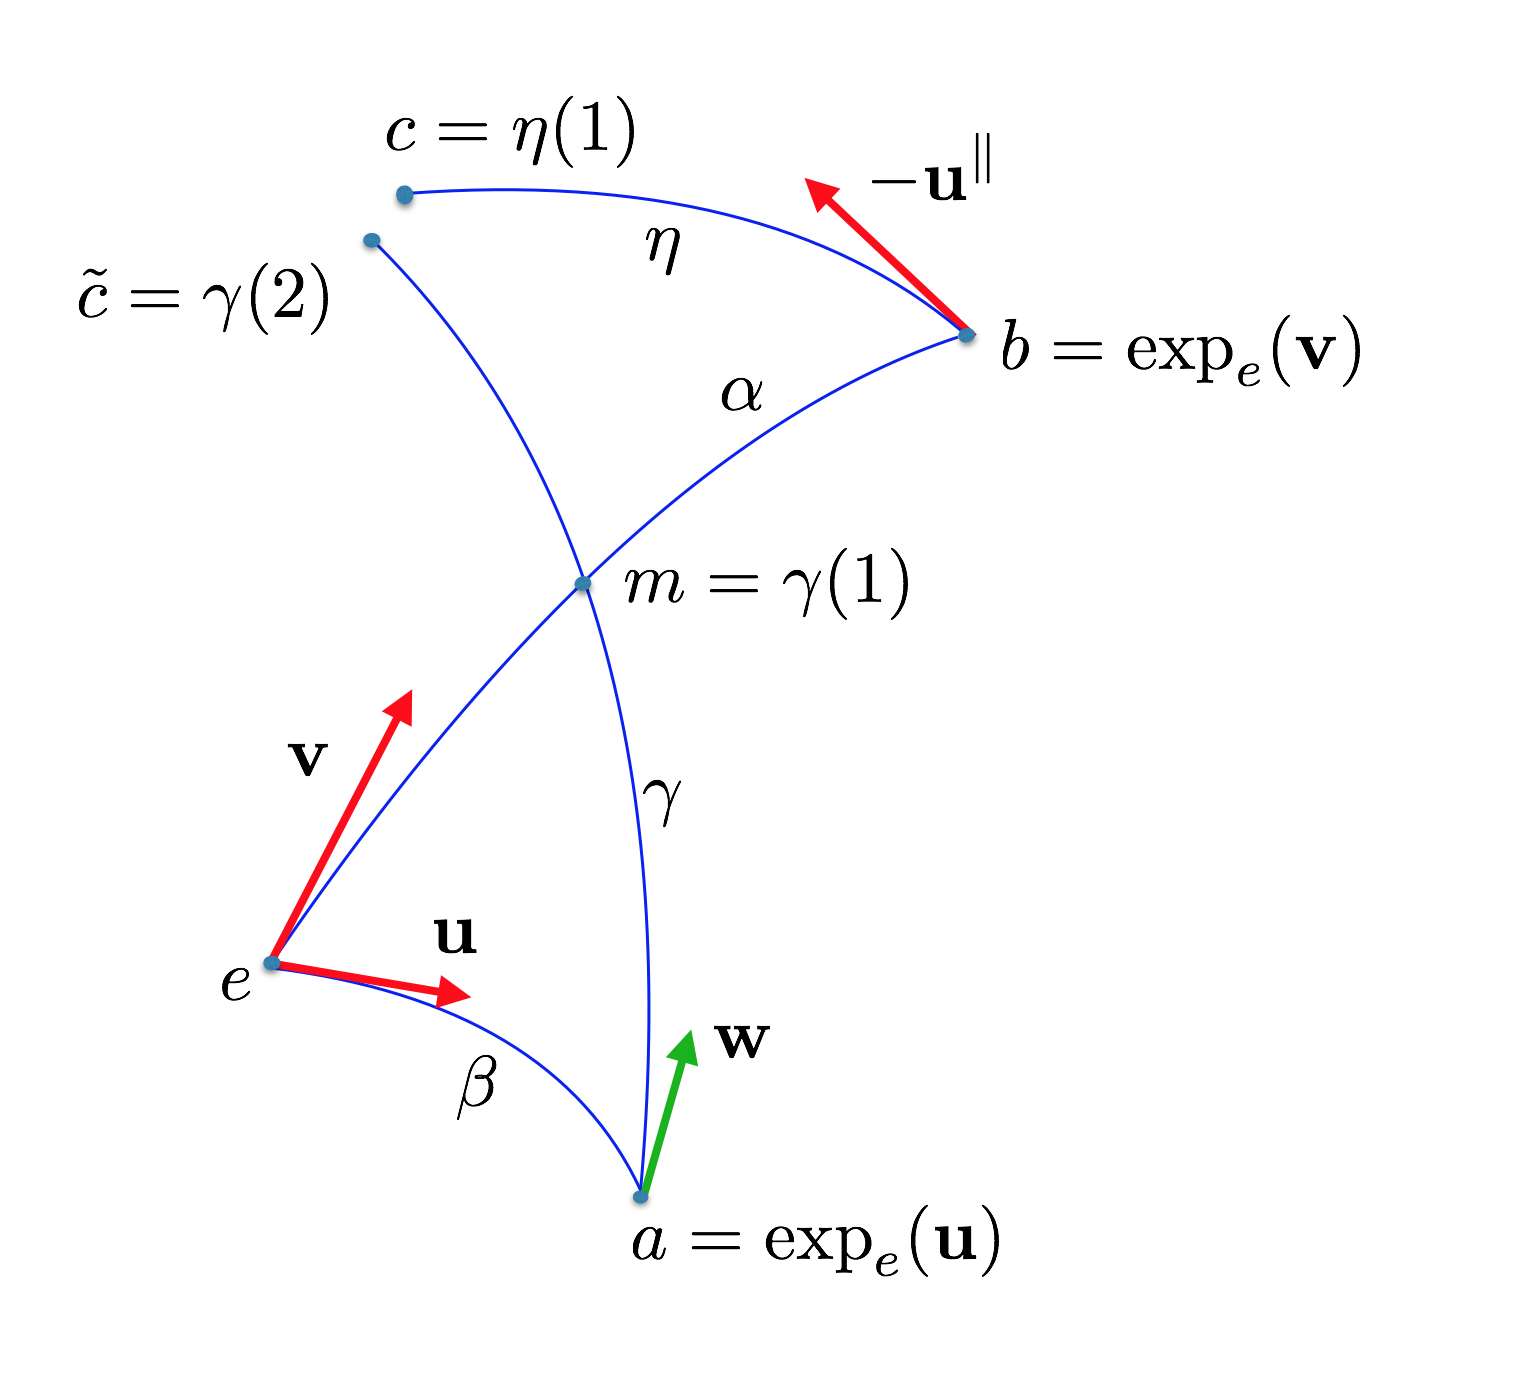
\includegraphics[width=9.5cm]{figures/theorem_pict.png}
	\caption{Pole ladder applied to parallel transport.}
	\label{fig:local}
\end{figure}

\begin{theorem}\label{th:local_approximation_theorem}
	Let $\mathbb{G}$ be a finite dimensional connected Lie group defined with a Cartan connection $\nabla$. 
	If, for each couple of linearly independent vectors $\mathbf{u}, \mathbf{v} \in T_{e}\mathbb{G}$, we consider the following elements:
	\begin{align*}
	a= \exp_{e}(\mathbf{u}) 
	\quad & \quad  
	b= \exp_{e}(\mathbf{v}) \\
	\mathbf{u}^{\parallel} = & \Pi(\alpha)_{e}^{b}(\mathbf{u})\\
	\gamma : [0,1] \rightarrow \mathbb{G} &\quad \gamma(0) = e \quad \dot{\gamma}(0) = \mathbf{v}
	\end{align*}
	Then, for $\mathbf{u}_{e}^{\parallel} := D(L_{b^{-1}})_{e}( -\Pi(\alpha)_{a}^{b}(\mathbf{u}))$, the approximation
	\begin{align*}
	\exp_{e}(\mathbf{u}_{e}^{\parallel}) 
	\simeq
	\exp_{e}\big(\frac{\mathbf{v}}{2}\big)   
	\circ  \exp_{e}(\mathbf{u}) 
	\circ \exp_{e}\big(-\frac{\mathbf{v}}{2}\big)
	\end{align*}
	holds.
\end{theorem}

\begin{proof}
	As a consequence of the construction we have the following considerations:
	\begin{align*}
	\gamma(t) &= \exp(t\mathbf{w}) 
	= 
	a \circ \exp_{e}(D(L_{ba^{-1}})_{e}(t\mathbf{w})) 
	= 
	\exp_{e}(\mathbf{u})  \circ \exp_{e}(D(L_{a^{-1}})_{e}(t\mathbf{w})) 
	\\
	m &= \alpha(\frac{1}{2}) 
	= \exp_{e}\big(\frac{\mathbf{v}}{2}\big) = \gamma(1) = \exp_{a}(\mathbf{w})
	\\
	\exp_{e}&(D(L_{a^{-1}})_{e}(\mathbf{w})) = \exp_{e}(-\mathbf{u}) \circ  \exp_{e}\big(\frac{\mathbf{v}}{2}\big) 
	\end{align*}
	Let $\eta$ be the integral curve of  $-\Pi(\alpha)_{a}^{b}(\mathbf{u})$ starting at $b$. If $c := \eta(1)$ and $\tilde{c} := \gamma(1)$, then on one side we have:
	\begin{align*}
	\tilde{c} = \gamma(1) &= \exp_a(2\mathbf{w}) = a \circ\exp_{e}(D(L_{a^{-1}})_{e}(2\mathbf{w})) \\
	&= \exp_{e}(\mathbf{u})\circ\exp_{e}(D(L_{a^{-1}})_{e}(\mathbf{2w})) \\
	&= \exp_{e}(\mathbf{u})\circ\exp_{e}(2D(L_{a^{-1}})_{e}(\mathbf{w})) \\
	&= \exp_{e}(\mathbf{u})\circ \big(\exp_{e}(D(L_{a^{-1}})_{e}(\mathbf{w})) \big)^2\\
	&=  \exp_{e}(\mathbf{u})\circ \big(  \exp_{e}(-\mathbf{u}) \circ  \exp_{e}(\frac{\mathbf{v}}{2}) \big)^2\\
	&=   \exp_{e}\big(\frac{\mathbf{v}}{2}\big)   
	\circ  \exp_{e}(-\mathbf{u}) 
	\circ \exp_{e}\big(\frac{\mathbf{v}}{2}\big) 
	\end{align*}
	On the other side:
	\begin{align*}
	c = \eta(1) &= \exp_{b}(-\mathbf{u}^{\parallel}) = b \circ\exp_{e}(D(L_{b^{-1}})_{e}(-\mathbf{u}^{\parallel})) \\
	&= \exp_{e}(\mathbf{v}) \circ\exp_{e}(D(L_{b^{-1}})_{e}(-\mathbf{u}^{\parallel})) \\
	&= \exp_{e}(\mathbf{v}) \circ\exp_{e}(-\mathbf{u}_{e}^{\parallel}) 
	\end{align*}
	where $D(L_{b^{-1}})_{e}(\mathbf{u}^{\parallel})$ has been written $\mathbf{u}_{e}^{\parallel}$ for brevity.
	If we consider $c\simeq \tilde{c}$ it follows that:
	\begin{align*}
	\exp_{e}\big(\frac{\mathbf{v}}{2}\big)   
	\circ  \exp_{e}(-\mathbf{u}) 
	\circ \exp_{e}\big(\frac{\mathbf{v}}{2}\big)
	\simeq
	\exp_{e}(\mathbf{v}) \circ\exp_{e}(-\mathbf{u}_{e}^{\parallel}) 
	\end{align*}
	which implies
	\begin{align*}
	\exp_{e}(-\mathbf{u}_{e}^{\parallel}) 
	&\simeq
	\exp_{e}(-\mathbf{v}) 
	\circ \exp_{e}\big(\frac{\mathbf{v}}{2}\big)   
	\circ  \exp_{e}(-\mathbf{u}) 
	\circ \exp_{e}\big(\frac{\mathbf{v}}{2}\big)
	\\
	\exp_{e}(-\mathbf{u}_{e}^{\parallel}) 
	&\simeq
	\exp_{e}\big(-\frac{\mathbf{v}}{2}\big)   
	\circ  \exp_{e}(-\mathbf{u}) 
	\circ \exp_{e}\big(\frac{\mathbf{v}}{2}\big)
	\end{align*}
	As a consequence of property of the signs inversion it follows that
	\begin{align*}
	\exp_{e}(\mathbf{u}_{e}^{\parallel}) 
	\simeq
	\exp_{e}\big(\frac{\mathbf{v}}{2}\big)   
	\circ  \exp_{e}(\mathbf{u}) 
	\circ \exp_{e}\big(-\frac{\mathbf{v}}{2}\big)
	\end{align*}
\end{proof} 

\begin{corollary}
	.... \\
	If, with previous notations, the condition (1) is an approximation
	\begin{align*}
	\exp_{C}(\frac{\mathbf{k}}{2}) = \exp(\mathbf{\xi})\circ \exp_{M}(\frac{\mathbf{k}}{2}) 
	\end{align*}
	for some $ \mathbf{\xi}$ in  $\mathfrak{g}$ such that $\parallel\mathbf{\xi} \parallel < \delta$
	then the approximation has error
	\begin{align*}
	O(\parallel \delta\mathbf{u}^{\parallel} \parallel^{2} )  
	+ O(\parallel \mathbf{u} + \delta\mathbf{u}\parallel^{3})
	+ \text{...something that must be investigated depending on } \delta
	\end{align*}
\end{corollary}

